
The method we employed using \CP\ can be understood in a four part
fashion, as depicted in \refFigure{fig:genView}. The first part, in
the upper level of the figure, shows the Selector, which selects a
set of values for the inlining parameters based on a strategy. The
second part, on the left, shows the Combined Profiling (\CP) process
applied to a program. The third part shows the execution test of a
compiled program. And, in the center of the figure rests the compiler.

\begin{figure}
  \centering
  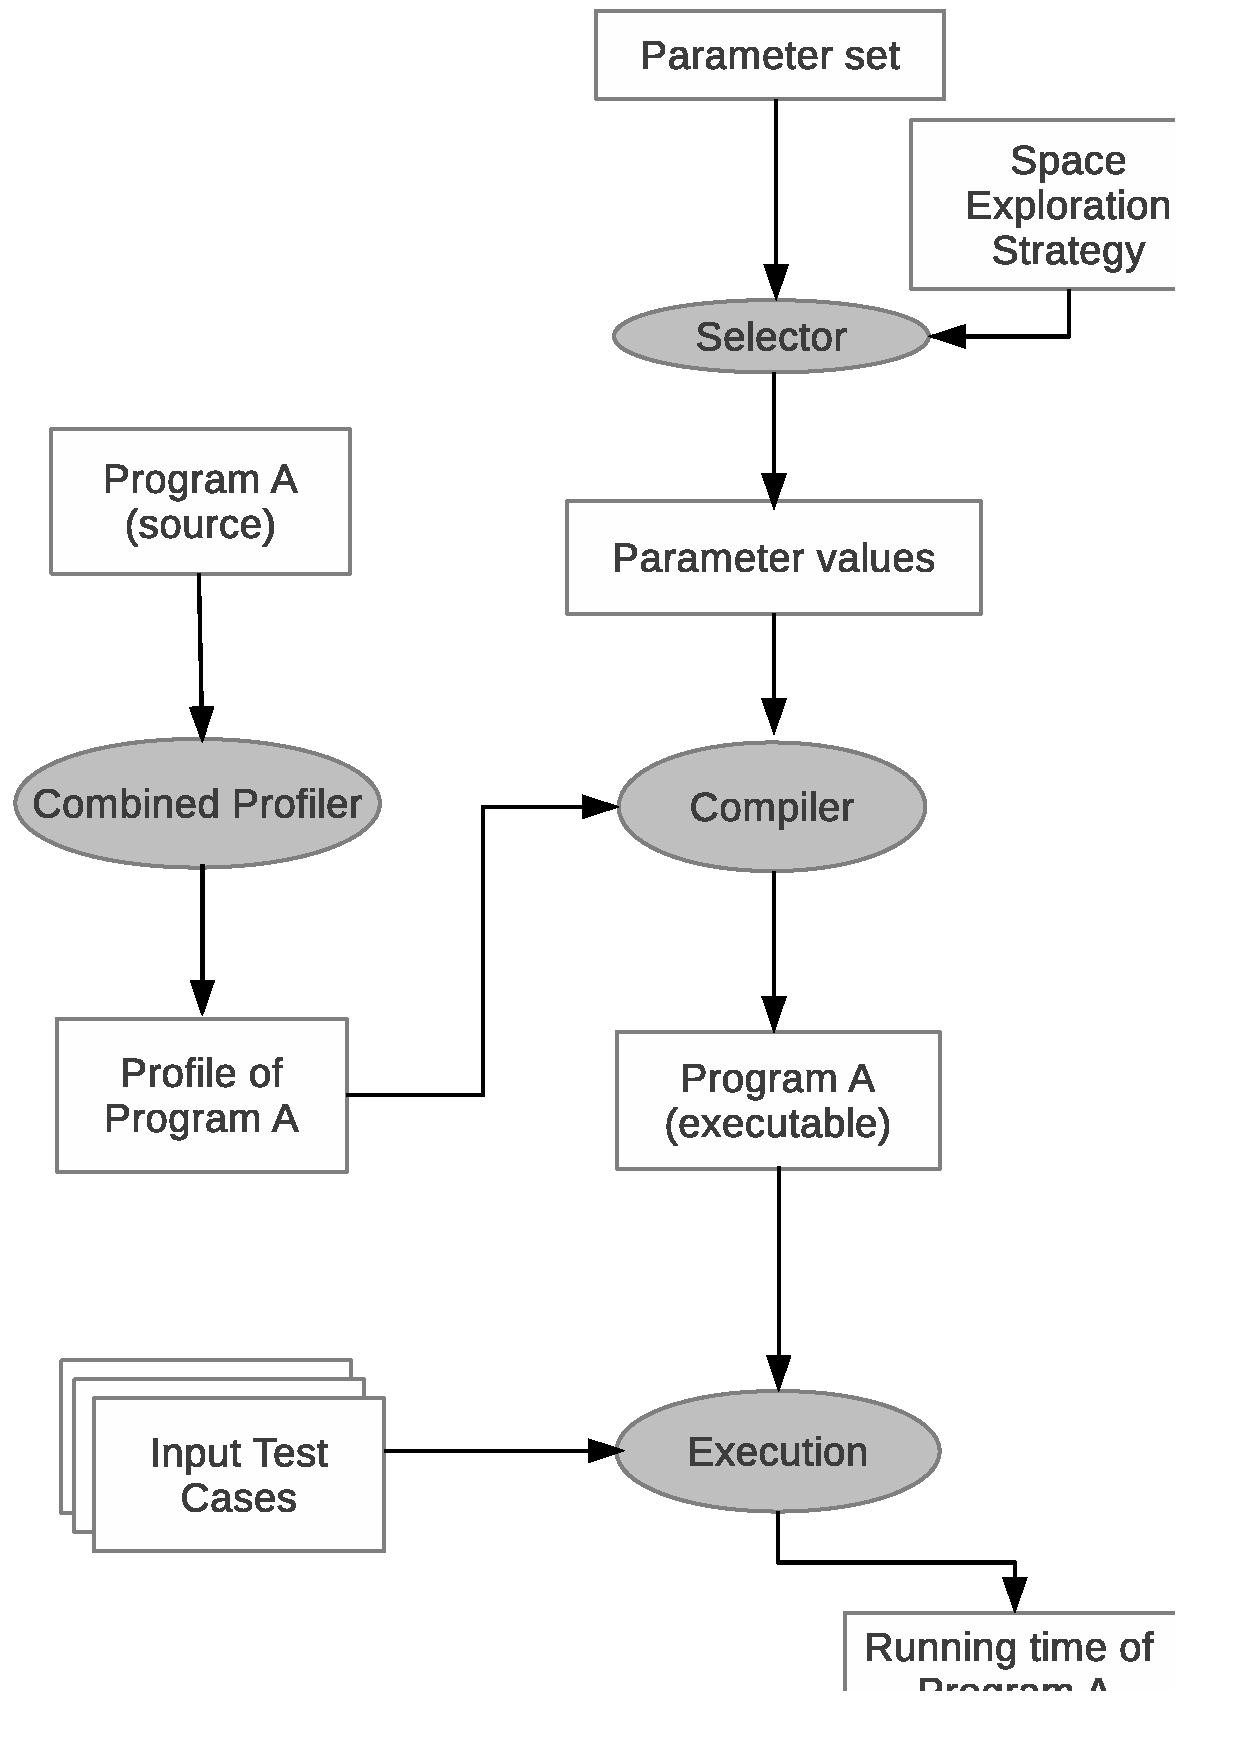
\includegraphics[width=0.50\linewidth]{Figures/genView}
  \caption{Generic view of the method}
  \label{fig:genView}
\end{figure}

We can use this method for parameter tuning, and also for a machine
learning approach trying to define the best set of parameters for
throughput or for latency. The process remains the same, we just have
to define properly what is a point of measure.

In the case of parameter tuning a point of measure is represented by
the set of parameter values of the compiler for the program under tuning
and its normalized value of the execution time for some test inputs. For
the machine learning case, a point of measure for throughput is the sum
of the execution times of some programs under test and its associated
parameter values. On the other hand, for latency a point of measure is
the geometric mean of the normalized values.

\subsection{Parameter Tuning}

Tuning the parameters of a compiler for a specific program 